%!TEX root = thesis.tex

\chapter{Introduction}
\label{chap:introduction}

\begin{chapquote}{Frederick Brooks, \textit{The Mythical Man-Month}, p.185}
``In spite of progress in restricting and simplifying the structures of software, they remain inherently unvisualizable, thus depriving the mind of some of its most powerful conceptual tools. This lack not only impedes the process of design within one mind, it severely hinders communication among minds.''
\end{chapquote}


Questions regarding how software interacts with the world and how
those that use the software benefit from it drive much of modern
software engineering research. As software becomes more ubiquitous,
the contexts in which we interact with it are becoming more diverse.
In many of these contexts, it is desirable to understand (at least to
some degree) what the software is \emph{doing}.

One interesting example of this trend is the artistic practice of
``live coding''\cite{TODO}, the artistic process of programming for
the entertainment or education of an audience. Source code is
projected on a screen an audience to observe, criticise or interact
with the programming process. Often the output is music or
graphics/visuals but the generation of these is always based in the
source code. Audience members at a live coding gig may have very
little experience in coding and not be able to comprehend or
appreciate live coding performances.

This presents both a challenge and an opportunity---how can the live
coder's software be presented so that an audience inexperienced in
programming can better appreciate the process of programming?

Software visualisation techniques have attempted to provide a higher
level of understanding of the structure of programs but have rarely
been effective in communicating the fundamental processes of software
development. \textit{The Mythical Man-Month} goes so far as to suggest
that ``software is invisible and unvisualizable''\cite{Brooks1995}
sparking debate as to the effectiveness of current software
visualisation techniques and whether software can be visualised at
all.

This thesis asks the question: ``can the application of software
visualisation techniques to live coding enhance audience experience by
increasing understanding and enjoyment?''. Through the development of
different software visualisations for live coding and by testing these
visualisations (through audience surveys) at real live coding
performances, it attempts to provide evidence-based conclusions while
remaining sympathetic to the fundamentally artistic goals of live
coding.

Live coding presents a unique application space for software
visualisation and the potential for effective communication directly
with audiences, potentially challenging this long-held belief that
``software is invisible and unvisualizable''.



% what is the problem

% state the problem more clearly

% make visualisation condition and visualisation techniques consistent throughout the thesis

% introduce live coding earlier

% audience experience in introduction

% art & science factors within this project - compromises are necessary to ensure the artistic factors are not removed

% don't reference mclean paper so much. discuss once, use results of discussion for making points

% Live coding, the artistic process of coding for an audience, has a problem.

% Live coding is the artistic process of programming for the entertainment or education of an audience. Source code is projected on a screen for audiences to observe, criticise or interact with the programming process. Often the output is music or visuals but the generation of these is always based in the source code.




\begin{figure}
\centering
\begin{subfigure}{.5\textwidth}
  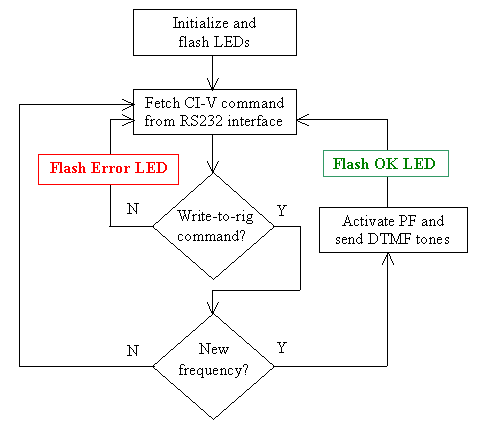
\includegraphics[width=.95\linewidth]{../images/code-visualisations/flow-chart.png}
  \caption{Flow chart}
  \label{fig:flow-chart}
\end{subfigure}%
\begin{subfigure}{.5\textwidth}
  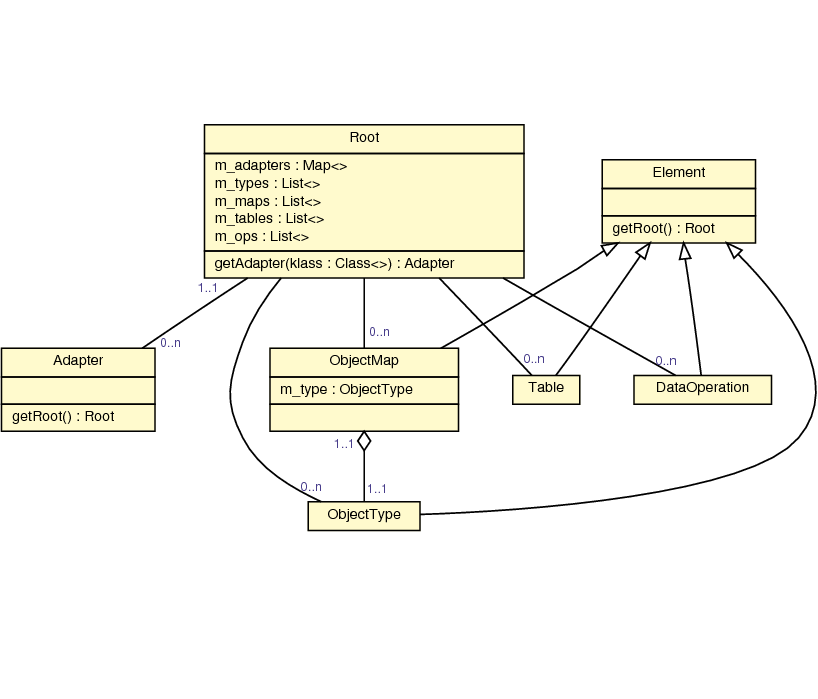
\includegraphics[width=.95\linewidth]{../images/code-visualisations/class-diagram.png}
  \caption{Class diagram}
  \label{fig:class-diagram}
\end{subfigure}\\
\begin{subfigure}{.5\textwidth}
  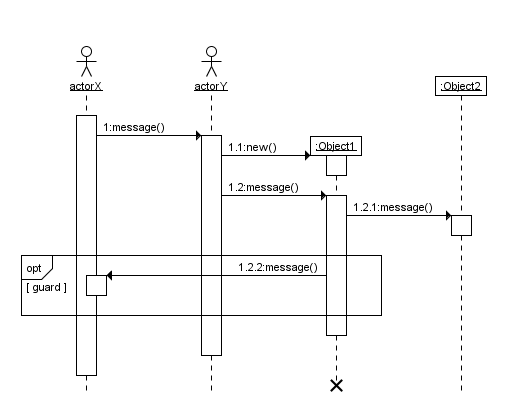
\includegraphics[width=.95\linewidth]{../images/code-visualisations/sequence-diagram.png}
  \caption{Sequence diagram}
  \label{fig:sequence-diagram}
\end{subfigure}%
\begin{subfigure}{.5\textwidth}
  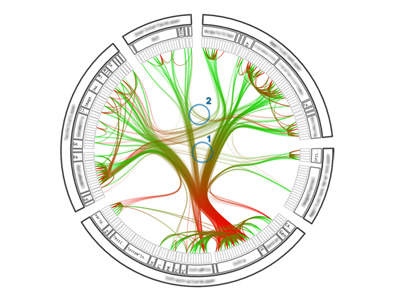
\includegraphics[width=.95\linewidth]{../images/code-visualisations/bundle-graph.jpg}
  \caption{Edge bundled graph}
  \label{fig:bundle-graph}
\end{subfigure}

\caption[Existing software diagramming and graphing techniques]{Existing software diagramming and graphing techniques.}
\label{fig:code-diagrams}
\end{figure}

\section{Background}

For most of its history, program source code has been displayed as simple text. This is due to the expressiveness of the text format and despite the inefficiencies of representing algorithms and abstractions in natural language.

Recently, due to ever increasing programming language complexity, increasing screen fidelity and increasing computational power, code annotations and syntax highlighting have become commonplace. Nevertheless, these visual enhancements rarely provide information beyond the basic grammar of the language they are intended to augment. The limitations of this approach are becoming ever more apparent as programming languages and interactive programming environments move towards the need for real-time comprehension and a need to understand the source code within the context of a running program.

Historically, source code diagrams have attempted to display the high level structure of source code. For example, class diagrams (see Figure~\ref{fig:class-diagram}) are commonly used to document the structure of a program whereas flowcharts (see Figure~\ref{fig:flow-chart}) have been used extensively to represent simple software behaviours. Sequence diagrams (see Figure~\ref{fig:sequence-diagram}) have allowed the visualisation of interacting objects and actors in a software system, putting the focus on the users of the software system rather than the structure of the program. Edge bundling of software call stacks~\cite{Zhou2013} (see Figure~\ref{fig:bundle-graph}) has allowed the visualisation of the lifecycle of a program, showing which software components were called at what time and the volume of calls made.

\subsection{Hotswapping Source Code}

Various modern software environments now support the concept of hotswapping source code. Within software environments, hotswapping refers to the process of modifying program source code at runtime to achieve desired behaviour without interrupting or restarting the system. Examples of languages and platforms supporting this workflow include Java with HotSwap or JRebel~\cite{ZeroTurnaround2014} and Python, in addition to a variety of other custom platforms and modifications (e.g.~\cite{Thomas2011}). This workflow has also inspired the programming practice of ``live coding''. 

Live coding further develops the concept of hotswapping source code, applying it to live musical and visual performance. In live coding a programmer performs for an audience. The audience observes the programmer as they modify an active program to produce music and visuals. Some of the most important and influential live coding environments over the last decade have included SuperCollider~\cite{McCartney}, ChucK~\cite{Wang2008} and Extempore~\cite{Sorensen}. These environments have a growing following as the field of live coding matures.

\subsection{Live Coding}

\begin{figure}
\centering
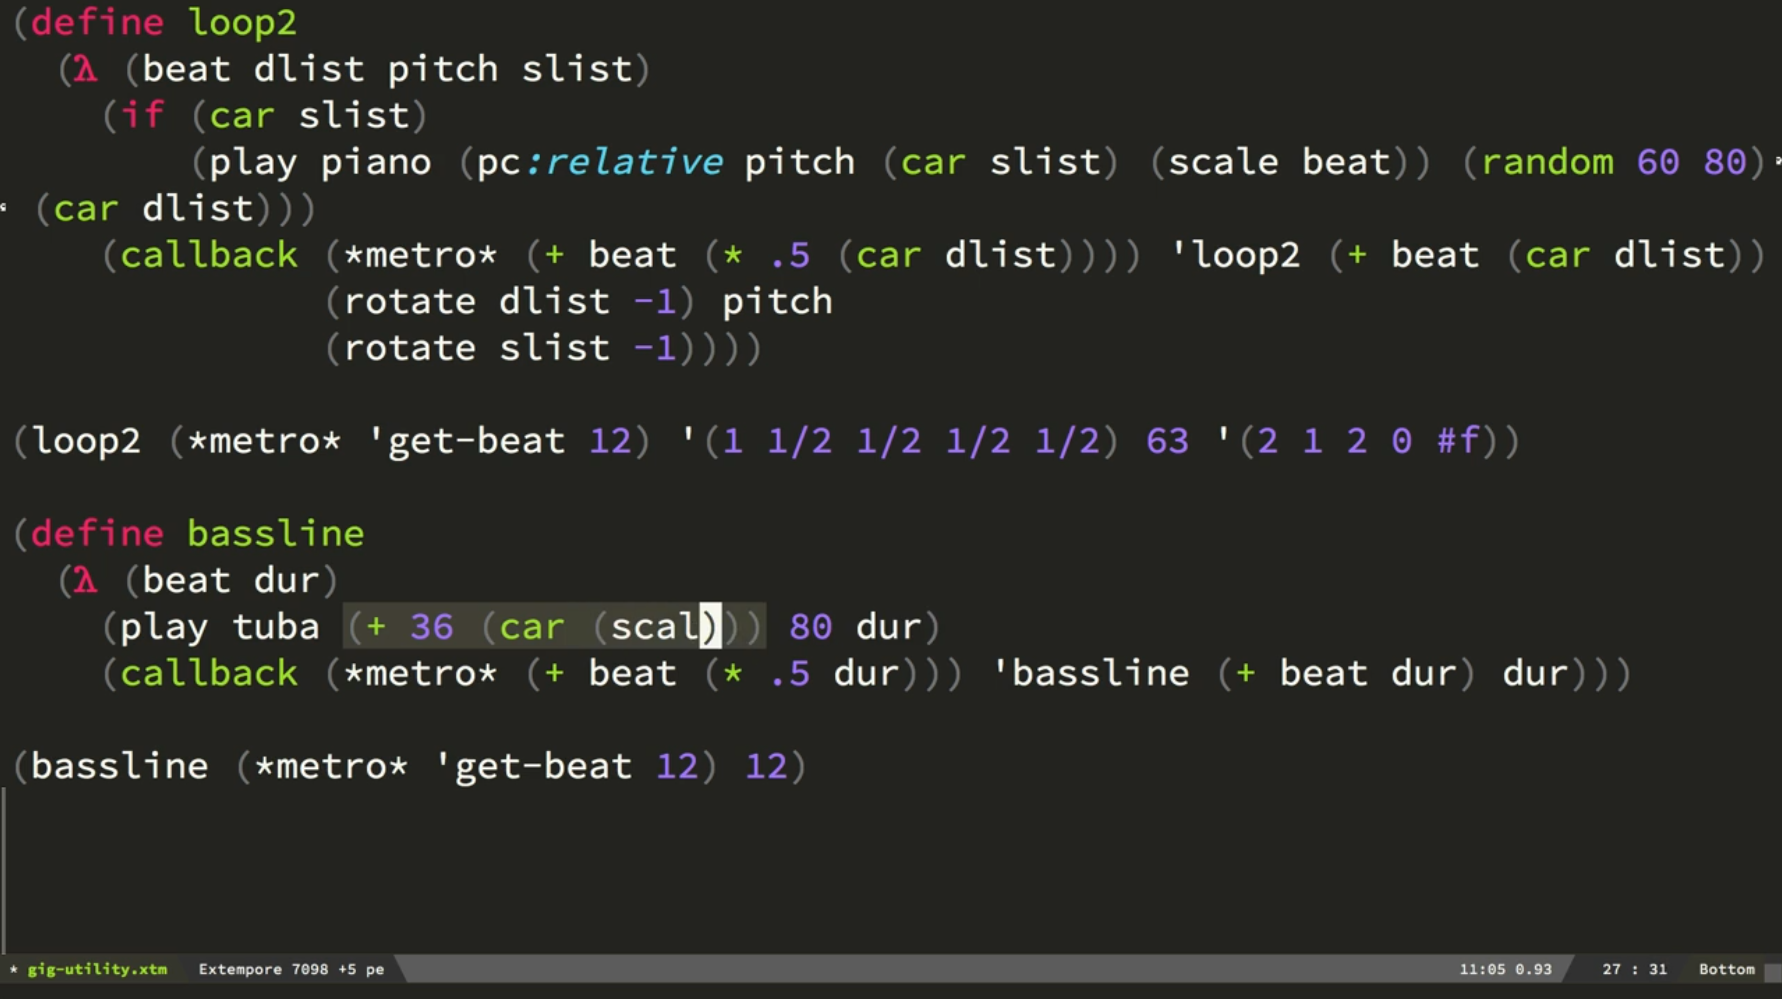
\includegraphics[width=1.0\textwidth]{../images/code/live-coding-screen.png}
\caption[A typical live coder projection]{A typical live coder projection includes the raw source code of the musical performance such as the screen pictured above. Audiences observe the changes to the source code on a projector screen while listening to the musical output. In the source code pictured here, the live coder is making changes to the musical ``bassline'' during a performance.}
\label{fig:live-coding-screen}
\end{figure}

% \begin{figure}
% \centering
% 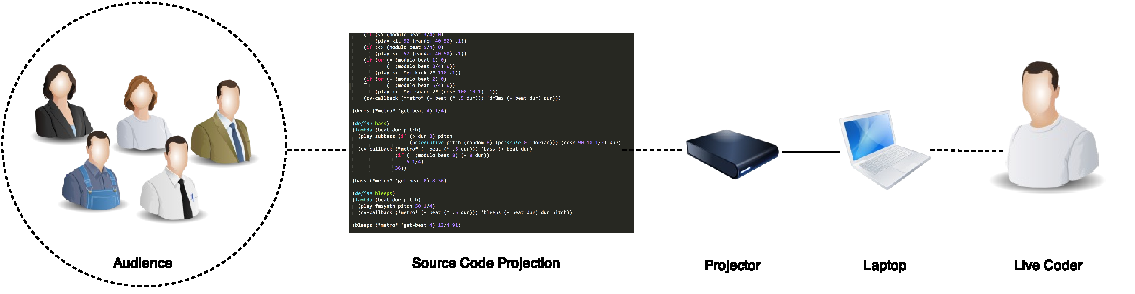
\includegraphics[width=1.0\textwidth]{../images/live-coding-setup.pdf}
% \caption[The live coding process]{Conceptual diagram of the live coding process.}
% \label{fig:live-coding-setup}
% \end{figure}

Live coding can be broadly defined as writing a program while it runs~\cite{Ward2004}. More specifically, live coding is identified as the artistic process of musical and visual expression through programming~\cite{Collins2003}. Figure~\ref{fig:live-coding-screen} shows the standard screen projected for a live coding audience. The audience views the raw source code and the programming process as the programmer makes changes to the source code.

Live coding emphasises the concept of \emph{liveness}, a concept covered comprehensively within the literature~\cite{Auslander,Masura2007}. Liveness is foundational to the performance aspect of live coding in which the mantra is ``show us your screens''~\cite{Toplap}, asserting that all live coders should display their raw program source code to the audience.

A unique opportunity is provided through live coding to combine both source code and software visualisation techniques~\cite{McLean2010a}. This is due to the approach of live coding involving effective sensory communication, a goal of transparency of the coding process, and direct manipulation and refinement of the running program.

Firstly, live coding is built around communicating visually and audibly. This extends beyond the physical process of programming. Human input is visible in the creative process, demonstrating a link between physical actions and artistic output \cite{Mclean}.

Secondly, live coding has a history of exposing audiences to source code with the goal of ensuring the transparency of the coding process~\cite{Collins2011,McLean2010a}. It provides a space in which there is a direct mapping from the human interaction with the source code to the musical or visual output~\cite{Mclean}. This relationship allows for visuals to map the interaction with the output.

Lastly, live coding allows for direct manipulation and refinement of the running program~\cite{Swift2013}. This provides the capacity for uninterrupted visualisation of the dynamic aspects of the program combined with the static nature of the source code. Similarly, manipulation and refinement of the running program allows for manipulation of the software visualisation~\cite{McLean2010a}.
%- what does this achieve?
%- how do visualisations apply... what can they achieve within this space

% {\color{red} Studies conducted into the communication of the live coding process suggest that audiences may have a sense of exclusion from the live coding performance.}

% discuss functions, callbacks and other details relevant to live coding eg. evaluation...

\section{Related Work}


\begin{figure}
\centering
\begin{subfigure}{.5\textwidth}
  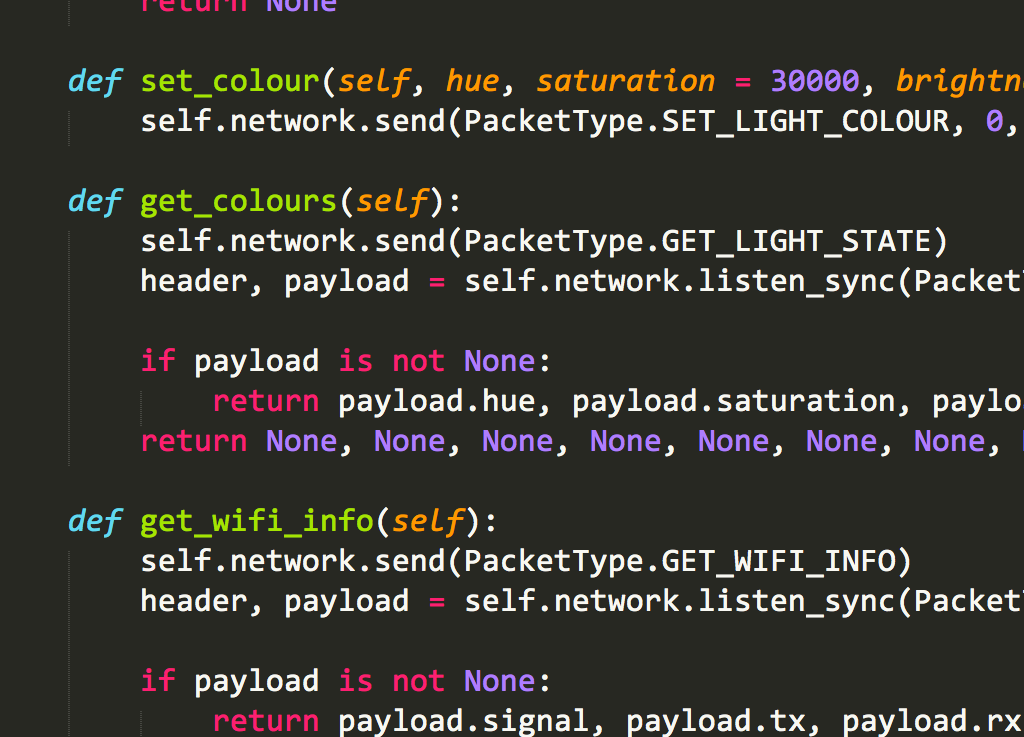
\includegraphics[width=.95\linewidth]{../images/code-visualisations/syntax-highlighting.png}
  \caption{Syntax Highlighting}
  \label{fig:syntax-highlighting}
\end{subfigure}%
\begin{subfigure}{.5\textwidth}
  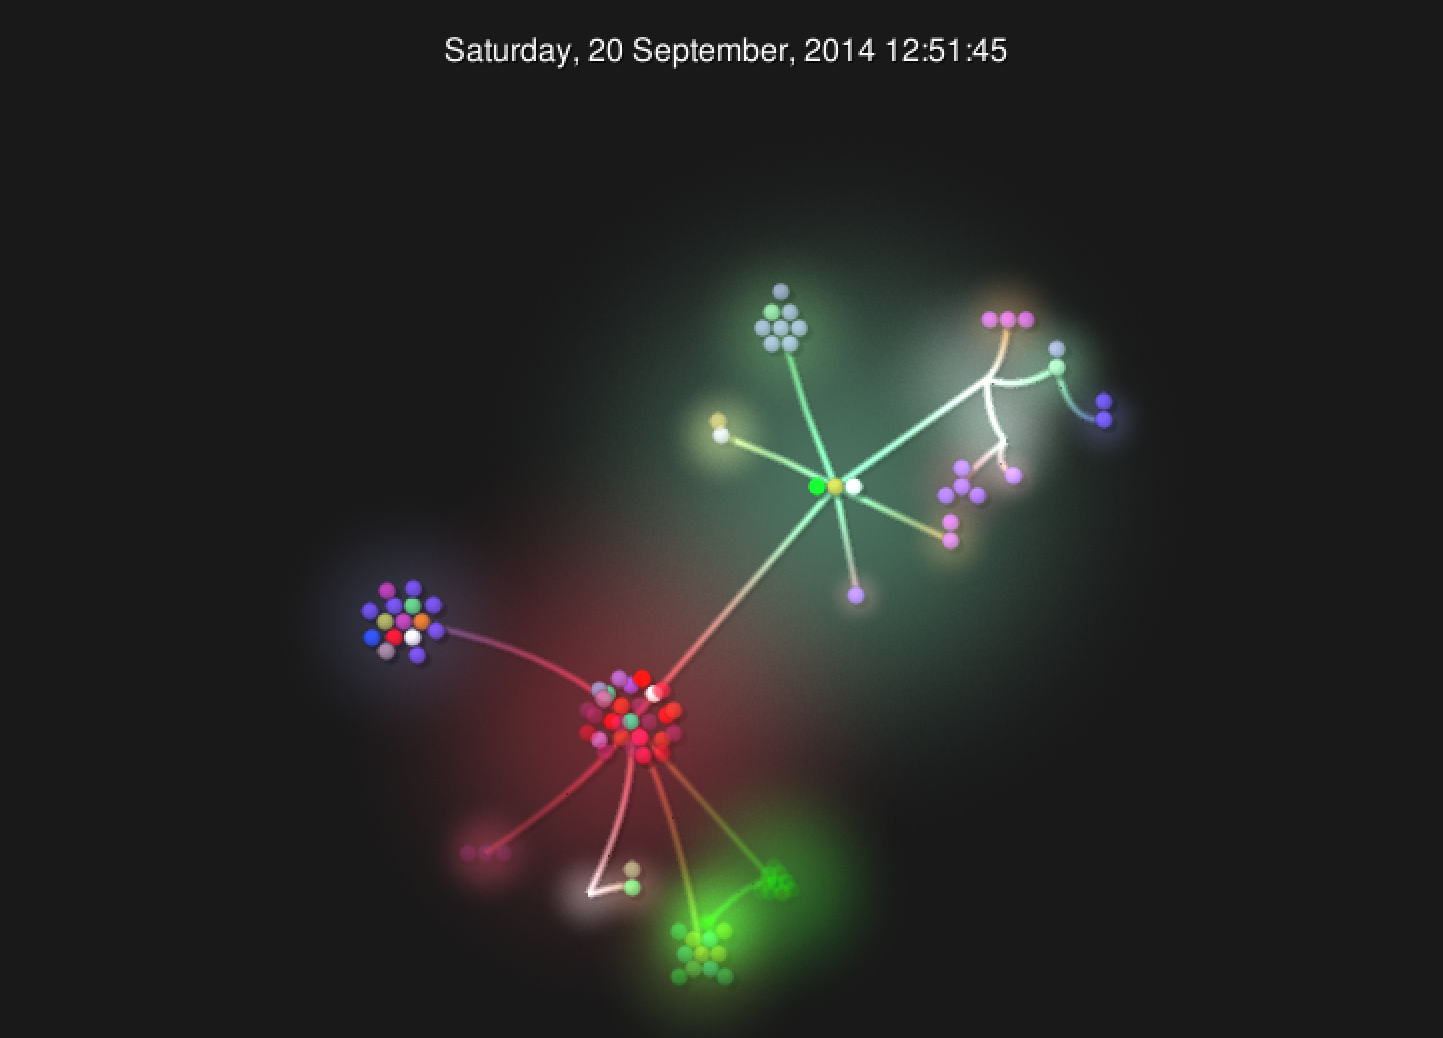
\includegraphics[width=.95\linewidth]{../images/code-visualisations/gource.png}
  \caption{Gource}
  \label{fig:gource}
\end{subfigure}\\
\begin{subfigure}{.5\textwidth}
  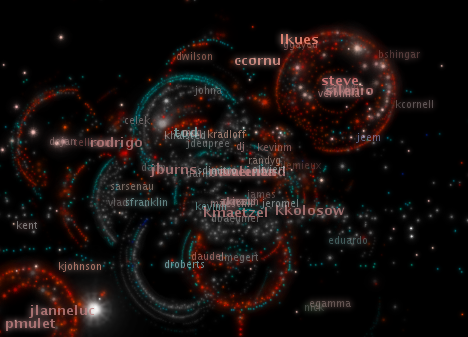
\includegraphics[width=.95\linewidth]{../images/code-visualisations/code-swarm.png}
  \caption{Code Swarm}
  \label{fig:code-swarm}
\end{subfigure}%
\begin{subfigure}{.5\textwidth}
  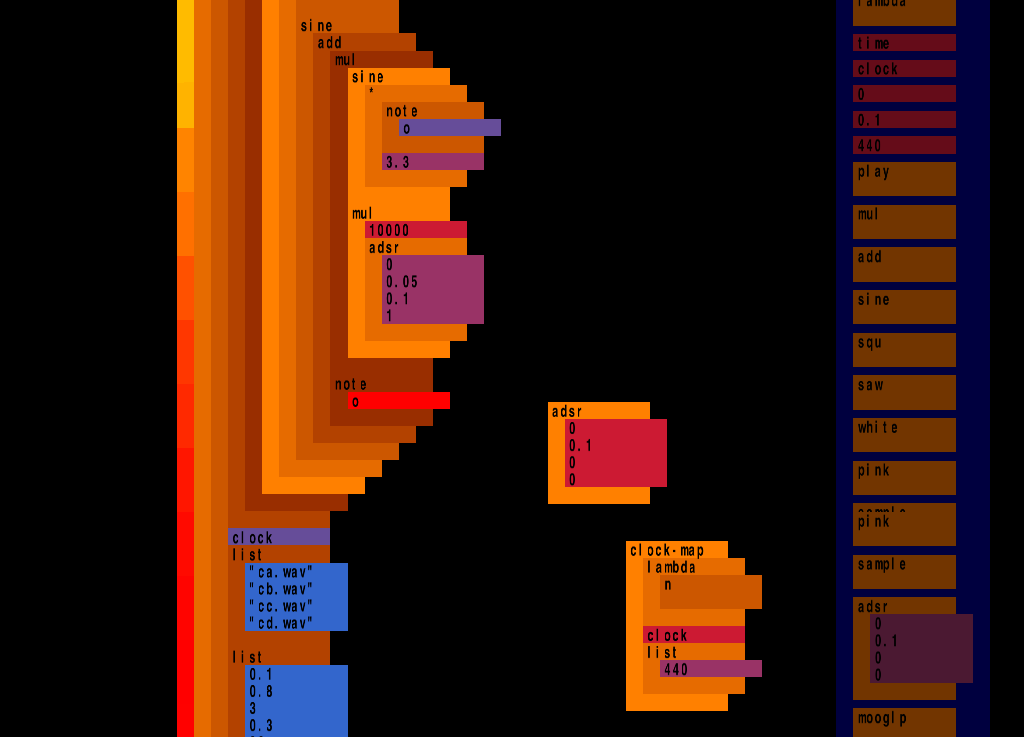
\includegraphics[width=.95\linewidth]{../images/code-visualisations/scheme-bricks.png}
  \caption{Scheme Bricks}
  \label{fig:scheme-bricks}
\end{subfigure}

\caption[Existing software visualisations techniques]{Existing software visualisations techniques.}
\label{fig:code-visualisations}
\end{figure}  

As noted above, a number of existing software visualisation techniques exist. Some of the most common software visualisations include static diagrams (see Figure~\ref{fig:code-diagrams}) and syntax highlighting (see Figure~\ref{fig:syntax-highlighting}). These techniques generally model the structure of the program to allow for more effective navigation around structures and take advantage of visual memory.

While diagrams and syntax highlighting provide information regarding the structure of source code, the fundamental nature of software is to change~\cite{Brooks1995}. Understanding these changes requires visualising the software development process. Techniques to visualise the changes occurring during the software development process include Gource~\cite{Caudwell2010} (Figure~\ref{fig:gource}) and Code Swarm~\cite{Ogawa2012} (Figure~\ref{fig:code-swarm}). These visualisation techniques show historic source code changes, based on source code repository data.

Showing historic source code changes allows the process of programming to be understood. However, this information is not immediately useful to programmers or observers. Visualisation of active software has shown potential in providing useful and interesting information, allowing the programmer to take actions based on the visualisations and allowing the observers to make relevant judgement of what actions the programmer is taking. Visualisation techniques such as inline annotations~\cite{Swift2013,Beck2013} provide direct feedback useful to both the programmer and observers, and technologies such as Light Table~\cite{Kodowa2014} with an inline interactive terminal and immediate visual feedback after hotswapping source code have further identified how useful visual feedback can be.

A number of attempts have been made in visualising active software within live coding. Examples of existing software visualisations within live coding include Scheme Bricks (Figure~\ref{fig:scheme-bricks}), Daisy Chain and Betablocker~\cite{McLean2010a}. These visualisation techniques suggest potential within live coding for effective process-driven visuals to enhance the observer's experience. However, no systematic studies of process-driven visualisations have been conducted within live coding.

% The art and science of live coding. The approach to evaluating the arts...
% The artistic nature of the live coding field cannot be ignored when evaluating the effect of aesthetic and didactic approaches on the enjoyment and understanding of the audience.
% -how does it relate to art?\\
% -why is it still a good approach for evaluating understanding.

\section{Structure}

This thesis discusses software visualisations which have been applied to live coding through a process of design iteration and evaluation in collaboration with a live coding artist. Three studies were administered, including one field study and two laboratory studies as a means to determine if understanding and enjoyment could be influenced by the introduction of visualisations to live coding.

Chapter~\ref{chap:literature-review} of this thesis summarises the literature including the basis for and the direction of this thesis. The current state of software visualisations and the state of the application of visualisations to live coding are examined with particular reference to the goals and future directions of the field.

Chapter~\ref{chap:exploratory-field-study} discusses the initial exploratory field study conducted to investigate existing perception and understanding of the live coding process. The field study explored the current state of live coding practice, examining the process of live coding, the effect on the audiences of live coding and the expectations of the audience.

Chapter~\ref{chap:visualisation-design} discusses the first iteration of the visualisation prototype developed following the results of the exploratory field study. The process of development is described with particular focus on software design within the space of an artistic process. This process involved collaboration with a live coding artist to develop software visualisations appropriate for the space of live coding.

Chapter~\ref{chap:user-study} summarises the initial user study conducted with the visualisation prototype. This study compared visualisation features in reference to enhancing the experience of the live coding audience. The study used surveys and video-cued recall techniques to examine live coding in the context of an artistic practice.

Chapter~\ref{chap:visualisation-refinement} discusses refinement of the visualisation prototype driven by the results of the initial user study. The initial user study identified a number of areas of improvement within the first iteration of the visualisation prototype and provided direction for following prototypes. The visualisation refinement took these concepts and applied them to the first iteration of the visualisation prototype.

Chapter~\ref{chap:follow-up-user-study} discusses the follow-up user study conducted to analyse the refined visualisations. A similar approach to the initial user study was taken, examining live coding audiences within the context of a live coding performance. However, in this case the examination compared the refined visualisation prototype with presenting just the plain source code within the live coding performance.

Chapter~\ref{chap:conclusion} summarises the results of the user studies, contributions, limitations and future work. Results of the field study and the two user studies are compared and the findings are discussed. Following this, the contributions made to the field of software visualisation and the visualisation of live coding are listed. Limitations with the contributions and limitations of the studies are then discussed. Future work in the field of software visualisation and the visualisation of live code is discussed with particular reference to developments of the methodology, improvements to the user studies and application spaces of the visualisation techniques discussed. A reflection on the process of combining a scientific approach with the arts is presented, followed by some closing words to conclude the thesis.


